\documentclass{article}


\usepackage{PRIMEarxiv}

\usepackage[utf8]{inputenc} % allow utf-8 input
\usepackage[T1]{fontenc}    % use 8-bit T1 fonts
\usepackage{hyperref}       % hyperlinks
\usepackage{url}            % simple URL typesetting
\usepackage{booktabs}       % professional-quality tables
\usepackage{amsfonts}       % blackboard math symbols
\usepackage{nicefrac}       % compact symbols for 1/2, etc.
\usepackage{microtype}      % microtypography
\usepackage{siunitx}
\usepackage{titling}
\usepackage{hyperref}
\usepackage{ragged2e}
\sisetup{per-mode=symbol}
\usepackage{lipsum}
\usepackage{parskip}
\usepackage{tabularx}
\usepackage{fancyhdr}       % header
\usepackage{graphicx}       % graphics
\graphicspath{{images/}}     % organize your images and other figures under media/ folder

%Header
\pagestyle{fancy}
\thispagestyle{empty}
\rhead{ \textit{ }} 

% Update your Headers here
\fancyhead[LO]{Aim Is All You Need}
% \fancyhead[RE]{Firstauthor and Secondauthor} % Firstauthor et al. if more than 2 - must use \documentclass[twoside]{article}

% Define the subtitle command
\pretitle{%
  \begin{center}
  \LARGE
}
\posttitle{%
  \par\vskip0.5em%
  \begin{large}
  \textsl{\thesubtitle}%  This prints the subtitle
  \end{large}\par\end{center}%
  \vskip1.5em
}
\newcommand{\subtitle}[1]{\def\thesubtitle{#1}}
  
%% Title
\title{Aim Is All You Need}
\subtitle{A Conceptual Introduction to Externally Pulsed Propulsion}

\author{
  Seth Katz \\
  \texttt{katzseth22202@gmail.com} \\
}

\newcolumntype{L}{>{\RaggedRight\arraybackslash}X}
\newcolumntype{C}{>{\RaggedRight\arraybackslash}c}

\begin{document}
\maketitle

\begin{abstract}\label{sec:abstract}
 In 2017, Google Research published ``Attention is All You Need" \cite{vaswani2023attentionneed}.  Their paper introduced the Transformer, which let neural networks capture long range dependencies.   Just a few years later, OpenAI developed tools like ChatGPT \cite{chatgpt} that resemble hypothetical early prototypes of the computers in Star Trek \cite{startrek}.

But here's the bittersweet truth:  While our screens flicker with progress, the tangible realms of space, energy and paleontology remain comparatively stagnant.

\textbf{Dude, Where's my spaceeship?}

This paper's goal is to enable our progress in physical realms to catch up with our progress online.  Our journey requires applying a single unifying idea that is much simpler than attention - aim.   \begin{figure}[htpb]
    \centering
    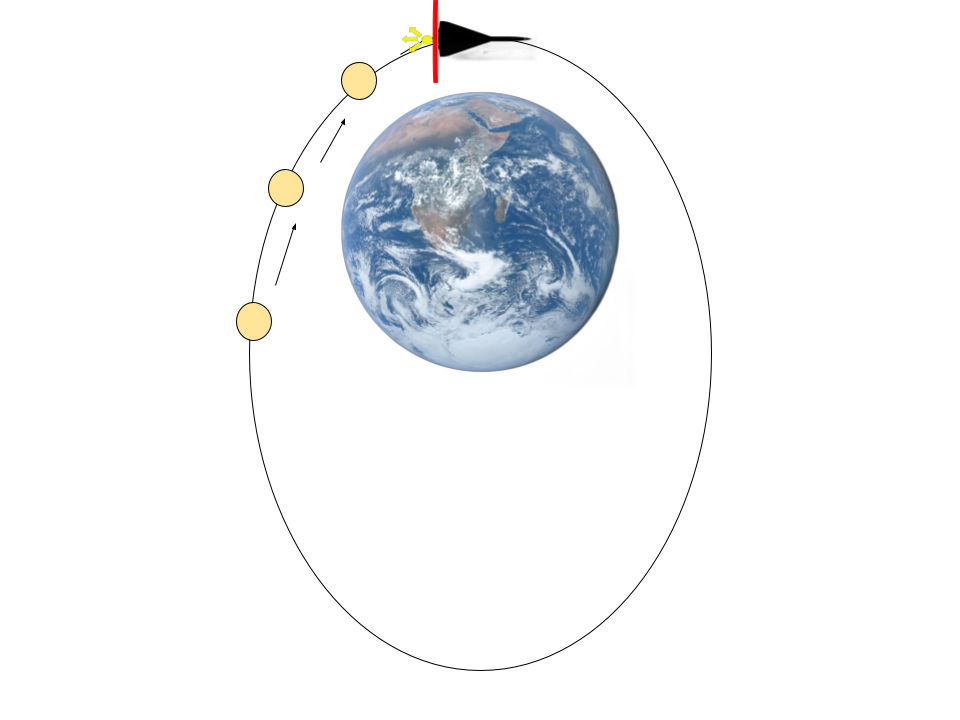
\includegraphics[width=0.5\linewidth]{images/Starship_Impact_ellipse.png}
    \caption{Balloons from a first rocket (not shown) crash into a second target rocket and provide propulsion \cite{earth_image}}
    \label{fig:balloon_impact}
\end{figure}

Consider two rockets.   The first deploys a series of fast moving low density balloons with miniaturized rockets capable of small navigation adjustments.  As shown in \autoref{fig:balloon_impact} these balloons precisely follow a path to sequentially crash  into a separate  target rocket.   These precise collisions deliver high-density jolts of pulsed energy and momentum to the target vehicle, enabling a surprisingly broad range of groundbreaking applications (See \autoref{tab:applications}).    

Paralleling their role in consumer AI, neural networks offer a promising avenue to extend current CubeSat formation flying algorithms with the precise control required for this externally pulsed propulsion.

\begin{table}[!htpb]
    \centering
    \caption{A Checklist of Grand Challenges Externally Pulsed Propulsion Can Solve}
    \label{tab:applications}
    \begin{tabularx}{\textwidth}{|c|L|}\hline 
        \textbf{Safer Satellite Launch} & We'll launch expensive satellites and astronauts without strapping them to fragile extremely high propellant mass fraction rockets.   See \autoref{sec:starship_safelaunch}. \\\hline
        \textbf{Suborbital Transit} & We'll create a viable suborbital travel vehicle allowing passengers to take off from normal airport runways and reach anywhere in the world in less than 2 hours. Noise pollution near population centers will be no worse than it is with conventional aircraft.  See \autoref{sec:200_mile_high}.\\\hline
        \textbf{Rocket Revolution} & We'll end the tyranny of the rocket equation. We'll still use small rockets, but giant rockets with high propellant mass fraction will no longer be needed to reach orbit. See \autoref{sec:no_isru_rocket}\\\hline
        \textbf{Lunar Lift-off} & Launching from the moon may still require volatiles, but not the more difficult task of making and storing high performance rocket fuel. \autoref{sec:lunar_rockets_no_fuel}\\ \hline
        \textbf{Jurassic Dark} & As a side effect of our advances, we'll create the field of lunar paleontology and discover concrete evidence for how life originated on Earth. We'll build a genetic record of extinct species from ancient geological periods, like the dinosaurs. See \autoref{sec:jurassic_dark} \\\hline
        \textbf{Straw Ways to Heaven} & We can construct terrestrial megastructures, extending from the ground to the edge of space, without relying on advanced magnetic technologies such as Lofstrom Launch Loops \cite{lofstrom_loop}. A particularly ambitious yet beneficial example might be a vacuum tube connecting Earth and space, a "Straw Way to Heaven."\\\hline
        \textbf{Carbon Cancelled} & We will solve our energy problems with carbon negative fuel that absorbs the carbon dioxide produced by industry, all while using minimal land and resources\\\hline
        \textbf{Moon mining} & We'll develop in-situ resource utilization (ISRU) technology, first on our moon (See \autoref{sec:lunar_mining}) and then on icy moons like Saturn's moon Phoebe\\\hline
    \end{tabularx}
\end{table}

Note, this paper summarizes some of the ideas in the blog ``Aim Is All You Need"\cite{aim2024}.
\end{abstract}

\section{Introduction}
Project Orion, conceived in the 1950s, remains the sole propulsion method based on mature contemporary technology that simultaneously offers specific impulse and thrust superior to chemical rockets \cite{projorion}. Orion would propel a spacecraft by directing hypervelocity plasma from nuclear explosions onto a pusher plate. Despite its theoretical promise, Orion faced insurmountable challenges related to political feasibility, radioactive fallout, and the impractical mass requirements stemming from the high minimum yield of nuclear explosions. Nevertheless, Orion conceptually validated the physics of hypervelocity pulsed propulsion.

Our approach replaces nuclear bombs with precisely aimed, hypervelocity gas balloons sequentially impacting a rocket's pusher plate. These balloons can be downscaled to practical sizes.  Unlike nuclear explosions, small hypervelocity gas impacts could be efficiently contained within a pulsed reaction chamber.

Leveraging gravity assists and the Oberth effect \cite{oberth_effect}, hypervelocity balloons could achieve high energy densities and specific impulses.  Recent cube sat formation flying and neural network advancements make the extremely precise navigation for this externally pulsed propulsion viable.  This paper presents a preliminary "back of the envelope" analysis, intended to establish the concept's potential. More rigorous, high fidelity analyses are reserved for future work.

\section{Groundwork and Prior Work for Externally Pulsed Propulsion}
\subsection{Navigation for Externally Pulsed Propulsion}
Millimeter accuracy CubeSat formation flying is rapidly advancing. The European Space Agency's (ESA) Proba-3 mission recently demonstrated this capability by creating artificial solar eclipses with a precise two CubeSat formation \cite{esa_proba_3}. The Stanford Space Rendezvous Laboratory's VISORS mission, nearing flight readiness (as of June 2025), will further showcase precise formation flying with an increased number of spacecraft \cite{guffanti2023autonomous}.  

Our hypervelocity balloons employ formation flying algorithms for precise positioning. We want to maximize gas mass and minimize the solid mass for mini-thrusters and electronics. To achieve this, a few coordinator CubeSats with enhanced computing and power will measure balloon positions and relay adjustment instructions.  As shown in \autoref{fig:coordinator-nodes}, these heavier coordinator nodes fly along with the balloons but do not impact the target rocket.  We keep the electronics on the balloons as simple and low mass as possible.   Each balloon, carrying perhaps a maximum of 100 grams of solid mass for sensors, power, mini-rockets, microcontrollers, and low-bandwidth communication with coordinator nodes, will detach its solid components shortly before hypervelocity rocket impact so they don't damage the target rocket.   Alternatively, the solids can fly through a small aperture in the pusher plate. Given that thousands of balloons are needed per mission, mass production will reduce costs.  

\begin{figure}
    \centering
    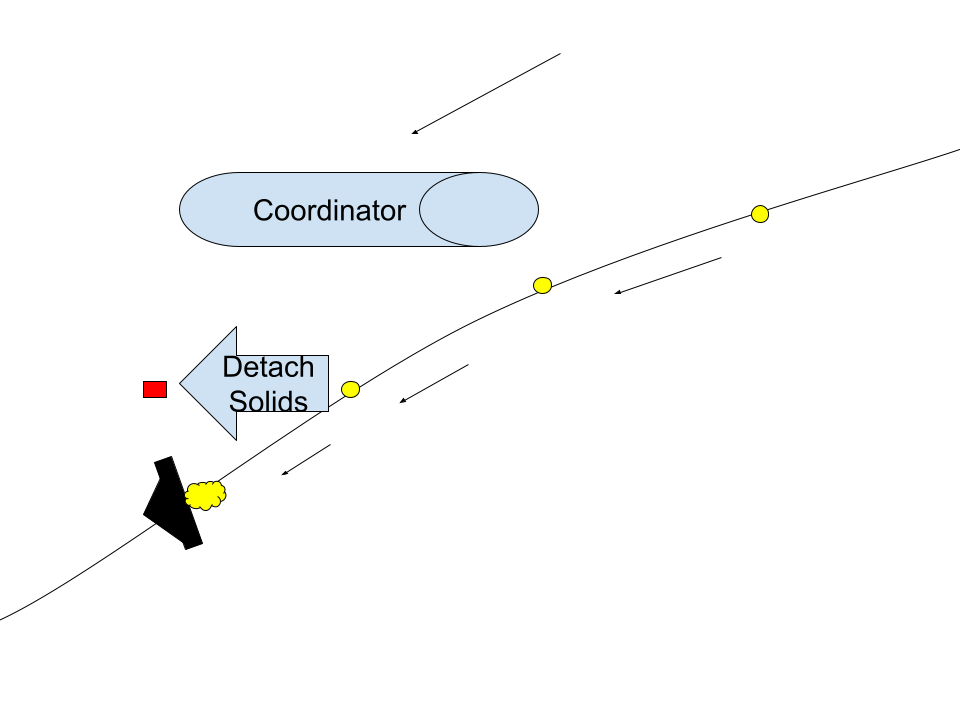
\includegraphics[width=0.5\linewidth]{images/Coordinator Nodes.png}
    \caption{Coordinator nodes that do not impact the spacecraft handle more complex measurement and computation.  Balloon solids can detach before spacecraft impact, or fly through a small aperture in the plate.}
    \label{fig:coordinator-nodes}
\end{figure}

Equipped with a high performance rocket based reaction control system, the target craft will precisely navigate and adjust its position to intercept each balloon in the formation.   Given the large number of balloons and high confidence in their relative positions, algorithms like Kalman filtering should enable precise state estimation for interceptions. After each balloon impacts the rocket, we'll need to rapidly adjust for any disparities between predicted and measured propulsion. This requires quickly solving for the necessary thrust adjustments to intercept the next balloon, all while adhering to the constraints on our rocket's performance. With thousands of balloons, the rocket's system must also be robust to occasional balloon failures caused by micrometeorite impacts or manufacturing defects. Neural networks show significant promise here because they can provide controllers with accurate initial guesses for trajectories \cite{guffanti2024transformerstrajectoryoptimizationapplication} and constraints \cite{briden_constraint}.   These good initial guesses produce fast convergence without compromising control guarantees.   Additionally, reinforcement learning shows promise for developing fast space trajectory recovery algorithms for anomalies like lost balloons \ \cite{zavoli2021reinforcement}.   This powerful combination of neural networks for rapid rocket adjustments and accurate formation flying can effectively keep the rocket on course for the next balloon interception.
\subsection{Mass Fraction of Balloon to Rocket Mass}
For externally pulsed propulsion to be a viable option, the ratio of balloon propulsion mass to rocket mass must be low for relevant rocket velocity changes. We develop a closed-form approximation for this ratio ( \autoref{eq:balloon_ratio} in {\autoref{sec:balloon_ratio_approximation}). Since real collisions are not perfectly elastic, our approximation includes an energy loss "fudge factor," \(e\).  Justification for a high \(e\) comes from Project Orion's findings \cite{orion_reflections}.   The Orion team found that pusher plate collisions could be opaque. This opacity implied minimal kinetic energy loss to pusher plate heating, resulting in a more elastic impact. Additionally, a curved, roughly parabolic pusher plate would produce a  highly collimated gas reflection. Therefore, we select a relatively high  \(e=0.8\).   

Relevant mass ratios and mission scenarios are summarized in \autoref{tab:mass_scenarios}. This table clearly shows that externally pulsed propulsion can lift significant mass into orbit. For instance, if a reusable rocket like SpaceX Starship \cite{starship} lifts 25 tons of balloons into a trans-lunar orbit, they can propel a 32 ton target craft into low Earth orbit. This exceeds the Space Shuttle's maximum capacity \cite{space_shuttle_program} or the zero fuel mass of smaller regional jets like the Embraer E170 \cite{embraer_e170}.

\begin{table}[!htpb] % tabularx should be inside a table environment
    \centering
    \caption{Mass Ratio of balloon to rocket with fudge factor \(e=0.8\)}
    \label{tab:mass_scenarios}
    \begin{tabularx}{\textwidth}{|p{4em}|p{4em}|p{4em}|p{6em}|L|}\hline
        \textbf{Rocket
        Final
        Velocity
        (\SI{}{\km\per\second})} & \textbf{Balloon
        Velocity (\SI{}{\km\per\second})} & \textbf{Rocket
        Initial
        Velocity (\SI{}{\km\per\second})} & \textbf{Rocket/Balloon
        Mass
        Fraction} & \textbf{Scenario} \\\hline
        7.784 & 10.916 & 0 & 1.28 & Eccentric balloons with apogee at lunar distance pushes rocket to minimal low Earth orbit\\\hline
        0 & 7.784 & 7.784 & 2.308 & Decelerate intercity rocket for powered reentry with retrograde balloons in low orbit \\\hline
        0 & 10.916 & 7.784 & 2.97 & Decelerate intercity rocket for powered reentry with retrograde balloons from lunar orbit \\\hline
        21.518 & 69.277 & 0 & 4.30 & Balloons approach Earth from Jupiter retrograde Hohmann trajectory and push the object to escape velocity and then to a periapsis near Parker Space probe \\\hline
        42.673 & 69.277 & 0 & 1.671 & Balloons approach Earth from Jupiter retrograde Hohmann trajectory and push the object to escape velocity and then to a periapsis near Parker Space probe but in a retrograde orbit around the Sun \\\hline
        3 & 6.421 & 0 & 2.54 & Launch balloons from the moon to trans-lunar injection orbit with low periapsis on Earth \\\hline
        0 & 2.58 & 2.38 & 2.17 & Decelerate trans-lunar payloads to land on the moon \\\hline
    \end{tabularx}
\end{table}

\subsection{Handling Space Debris}
The solid components of each balloon risk becoming space debris. To avoid this, we can intercept the balloons prior to their orbital periapsis.  For example, a balloon interception at a 200 kilometer altitude likely follows a predictable trajectory with negligible atmospheric drag.   If the balloon periapsis is near 100 kilometers, this likely deorbits any solid components.   They ideally then burn up or fall over remote oceans.   Two other techniques prevent long lasting space debris:

\begin{itemize}
\item The J2 perturbation induces a changing argument of periapsis. Any balloon orbit designed to avoid specific critical angles will eventually have a periapsis over the equator.  Since the Earth is wider at the equator, periapsis will be at a lower atmospheric altitude with much more drag.
\item If our balloon interceptions occur at night, subsequent daytime periapsis will be over a warmer atmosphere with higher drag at the same altitude.
\end{itemize}

\subsection{Balloon Deployment Details for Low Earth Orbit Scenario}
Let's consider the complexities of launching target rockets into Low Earth Orbit (LEO) with propulsion from balloons deployed in highly eccentric Earth orbits.

It's crucial to acknowledge that these balloons will not follow strictly identical Keplerian orbits. As the target rocket accelerates, the optimal balloon interception point moves along with it, so that successive balloons have slightly different orbital elements.
For low-density balloons, solar radiation pressure will significantly distort their orbits. To simplify orbit planning and maintain consistent  effects across the fleet, it's ideal for each balloon to remain outside the shadow of the others. This may necessitate slight variations in orbital parameters, such as inclination, for nearby balloons. The micro thrusters on each balloon  make corrections for unmodelled perturbations.  We still ensure each balloon achieves the correct interception position with the target rocket.   

Fortunately, strategically deploying our balloons near apoapsis can minimize the $\Delta v$ required for these inclination changes. Apoapsis balloon deployment also minimizes the $\Delta v$ for appropriate balloon spacing. The small $\Delta v$ changes required at apoapsis should enable practical designs for a very precise mechanical balloon launcher onboard our balloon deployment rocket.

Low density gas would consume too much volume in a balloon deployment vessel.   Instead, the balloons can be frozen and thaw once deployed from the rocket.  
\section{To The Moon by Water Balloon:  The Business Case for Externally Pulsed Propulsion}   
\subsection{Making Starship's Excess Capacity Useful To Satellite Customers} \label{sec:starship_safelaunch}
SpaceX's Starship may be the first fully reusable rocket. At scale, this could dramatically reduce space flight costs.   However, the rocket's large payload size is probably too big for today's space industry needs. For example, in \textit{The New York Times}
\begin{quote}
Carissa Christensen, the chief executive of Bryce Tech, an analytics firm that tracks the launch market, says launching Starship frequently will be key to closing SpaceX’s business case, but finding customers to fill the rocket’s giant payload capacity will be challenging. 
"Starship's payload capacity is huge; it's very, very big, and there aren't that many commercial uses today for a rocket that big," she said.  "Maybe it'll be so cheap that it makes sense to launch satellites on it if its not full or near full."  \cite{nyt_starship_size}
\end{quote}
Although many satellites might be too small to fill up Starship, they can still be very expensive to build and test. For an extreme example, the James Webb Telescope \cite{james_webb_space_telescope} cost \$9.7 billion dollars \cite{jwst_cost} to build. \textit{McKinsey Consulting} argues 
\begin{quote}
Safety and reliability will continue to be overarching concerns, suggesting excellent execution will be table stakes for a competitive launch company. \cite{mckinsey_reliability}
\end{quote}
Once rockets start ferrying astronauts, reliability becomes even more emphatically non-negotiable. Fully stacked, Starship weighs \SI{5}{\kilo\tonne} at launch \cite{starship}, yet its empty mass is only \SI{300}{\tonne}. That’s an awfully thin soda can strapped to a \SI{5}{\kilo\tonne} bomb that we're entrusting with billion-dollar satellites or human passengers.

By contrast, a suborbital rocket that merely reaches 200 kilometers in altitude might have a propellant mass fraction under 50 percent. This greater structural margin allows for more robust, reliable engines and extensive payload protection systems. Of course, such a suborbital rocket cannot reach orbit on its own.  It needs Starship to "push" it with externally pulsed propulsion.
\begin{figure}[htpb]
    \centering
    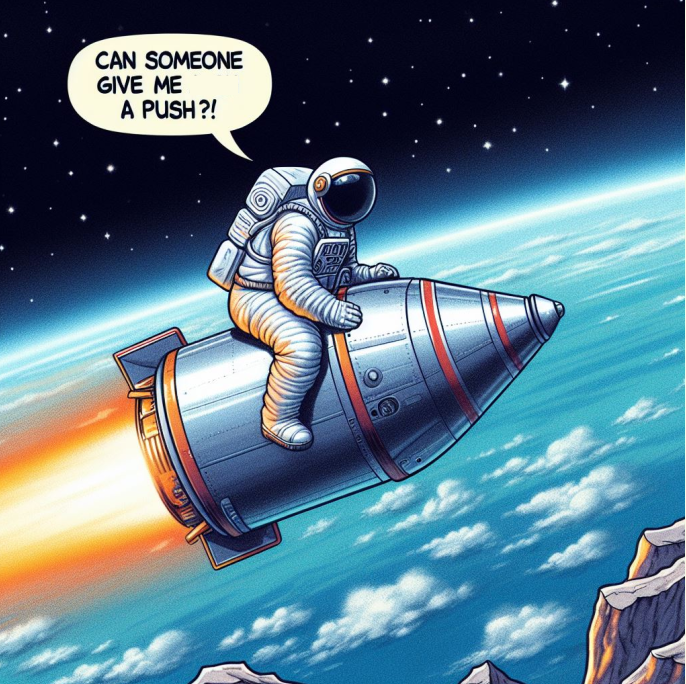
\includegraphics[width=0.5\linewidth]{images/suborbital_push_cartoon.png}
    \caption{A fun and of course very technically accurate cartoon about a suborbital rocket's $\Delta v$ limitations}
    \label{fig:suborbital-cartoon}
\end{figure}



Starship launches balloons for externally pulsed propulsion into a highly eccentric orbit around Earth, with a low 200-kilometer perigee and a high apogee. These balloons move near Earth’s escape velocity at perigee. The suborbital rocket intercepts the balloons with its pusher plate and rides their momentum pulses to low Earth orbit. While this approach reduces payload capacity compared to a single rocket system, most satellites are unable to take advantage of Starship’s enormous payload volume anyway.

\subsection{The 200 Mile High Club} \label{sec:200_mile_high}
SpaceX proposes direct Earth-to-Earth travel \cite{earth_to_earth}, ballistically launching passengers directly between cities with Starship from offshore platforms. This idea faces significant challenges:
\begin{itemize}
\item Marine environmental impact: Noise pollution from sea launches could severely harm marine ecosystems, including dolphins and whales.
\item Noise over populated areas: Starship's descent would generate loud sonic booms over cities.
\item Logistical inefficiency: Offshore launch platforms, by necessity located far from land, would add hours to the journey for boarding and departure, undermining the benefit of rapid travel.
\end{itemize}
A suborbital rocket plane offers a more practical alternative. To reach orbit, the suborbital rocket requires propulsion balloons launched by the Starship.   Starship can be launched from remote locations where noise pollution is acceptable.  Our suborbital rocket plane could take off from conventional urban airports using standard aircraft engines, then switch to rocket propulsion at high altitudes over remote areas to "skip" above the atmosphere and intercept Starship's propulsion balloons.   While normal airports can handle kerosene or methane fuel, most lack the infrastructure for cryogenic liquid oxygen.

However, two solutions address the liquid oxygen challenge:
\begin{itemize}
\item \textbf{Air-breathing Scramjets (Optimistic Scenario):} If economical passenger scramjets become feasible, rockets could accelerate to around Mach 7 before a steep climb, eliminating the need for liquid oxygen. This would also reduce propellant mass. Unfortunately, the extreme stress on the airframe makes suborbital rockets more economically viable for the foreseeable future.
\item \textbf{Mid-air oxygen refueling:} Suborbital rocket planes could receive liquid oxygen from specialized aircraft launched from airports equipped with liquid oxygen storage. This avoids retrofitting every urban airport, requiring only a single, strategically located airport near major destinations.   Mid-air refueling also reduces our rocket plane's takeoff weight.
\end{itemize}

A formation of propulsion balloons launched in an eccentric Keplerian orbit could only propel the  rocket plane on trajectories that bisect the Earth. Since most urban destinations would not align with such trajectories, the rocket plane needs to fire an adjustment burn at least once to reach the destination. Alternatively, a second set of propulsion balloons could intercept the rocket plane mid-flight and adjusting it's trajectory. Furthermore, to avoid a sonic boom upon descent, the plane must decelerate before atmospheric reentry. This deceleration could be provided by yet another set of propulsion balloons that were traveling in a retrograde orbit relative to the plane. Notably, these reentry balloons could be in a circular low Earth orbit rather than a high eccentricity orbit, significantly reducing the mass required.

\section{I Love ISRU.  Cheaper Externally Pulsed Propulsion \textit{Without} Giant Reusable Rockets}
For externally pulsed propulsion to achieve genuine economic competitiveness, the cost of launching its propulsion balloons must be exceptionally low.  The rocket plane must be robust enough to guarantee on-time takeoffs and avoid missing its initial balloon rendezvous.  Rocket acceleration must be limited for infants and other susceptible passengers, further increasing costs and $\Delta v$.  Even highly reusable rockets may prove too expensive, limiting this technology primarily to the very high-end private luxury aviation market. While luxury aviation customers typically prioritize flexibility, balloon-propelled flights necessitate advance scheduling.  Despite these limitations, the potential market for affluent travel between cities like Dubai and Dallas is likely at least an order of magnitude larger than the satellite market.

Still, it would be disappointing if we can't make suborbital travel mainstream.   If we can launch our balloons without giant rockets, we can reduce cost.   After all, "the best part is no part," \cite{best_part_no_part} and a reusable rocket is one heck of a part.

\subsection{Lunar Volatiles for Externally Pulsed Propulsion}

\begin{figure}[htbp]
    \centering
    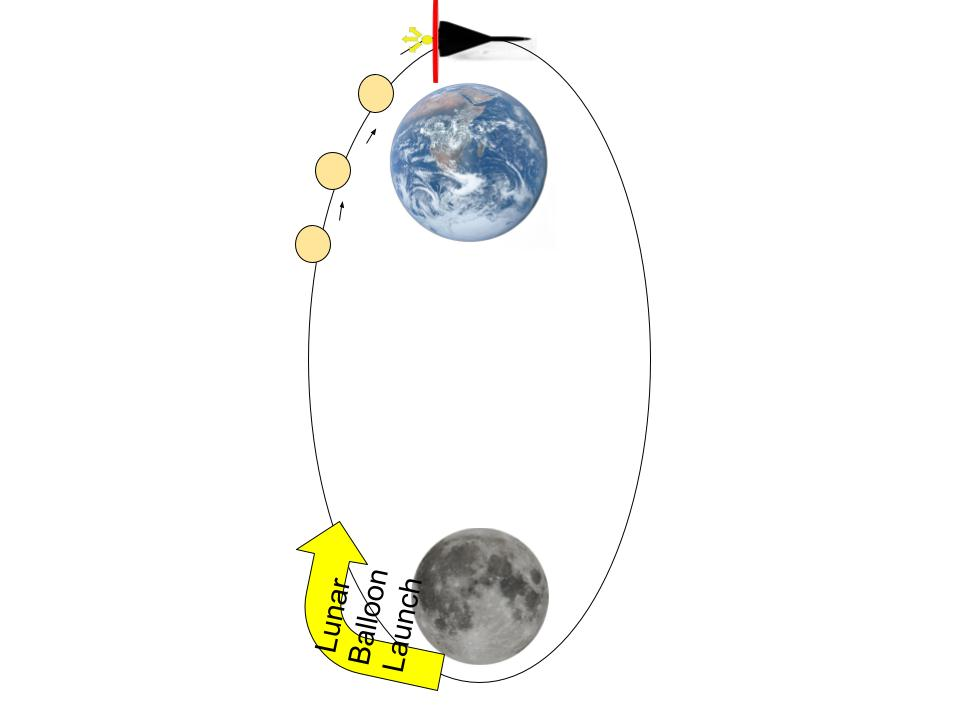
\includegraphics[width=0.5\linewidth]{images/Water Drawing From Moon.jpg}
    \caption{Lunar launched balloons replace Starship launched balloons \cite{earth_image} \cite{moon_image}}
    \label{fig:lunar_launched_balloons}
\end{figure}
Instead of using Starship, lunar volatiles extracted from the moon's permanently shadowed regions could fill our propulsive balloons. As shown in \autoref{fig:lunar_launched_balloons}, these balloons could be sent into a trans-lunar injection orbit that intersects our terrestrial suborbital rocket plane. Although balloon skins and electronics would likely still be sourced from Earth, volatiles constitute the majority of the balloons' mass. One approach to launching these balloons into orbit involves using rockets powered by lunar-derived propellants. The space community is enthusiastic about water electrolysis to produce and store cryogenic fuel for lunar rockets \cite{nasa_water}. However, this process is energy-intensive and requires complex cryogenic infrastructure, particularly for hydrogen fuel. Moreover, a reusable lunar rocket designed for repeated landings would require approximately \SI{6}{\km\per\second} of $\Delta v$, necessitating propellant mass fractions of about 75\% for hydrogen or 81\% for methane. While these figures are an improvement over Earth-launched rockets, the high propellant mass fractions remain a significant challenge.   

\subsection{Lunar Rockets without Lunar Rocket Fuel} \label{sec:lunar_rockets_no_fuel}
Instead of launching our lunar volatiles towards Earth with conventional rocket fuel, we launch off the moon using the same externally pulsed propulsion we've been discussing for terrestrial launches.   A rocket launched with externally pulsed propulsion from the lunar surface into a trans lunar injection orbit can burn its engines at periapsis around Earth.  Due to the Oberth effect, a small burn near Earth returns the rocket to the moon with a large velocity change.  As the rocket approaches the moon, it deploys its payload of balloons previously filled with lunar volatiles.  These returning balloons can push a new, more massive rocket filled with fresh volatiles off the moon.   We can then repeat this  cycle for exponential growth in lunar balloon launch mass capacity.   We've reduced combustible fuel requirements by burning our rockets near Earth.

However, we ideally don't want to make any chemical rocket fuel at all.   Let's again use external propulsion to launch our balloon deployment rocket from the lunar surface into a trans-lunar orbit.   We also launch a second set of balloons from the lunar surface into a retrograde trans-lunar orbit.   Using the millimeter precision navigation techniques we've discussed, we sequentially collide these retrograde balloons with more massive prograde balloons the main rocket is carrying.  We trap the exploding gas from these collisions in a pulsed reaction chamber and redirect this gas for thrust.    

If our colliding balloons each travel at $v=\SI{11}{\kilo\meter\per\second}$, then from \autoref{eq:max_m_rb} derived in \autoref{sec:dv_effective},  the maximum theoretical combined effective \(\Delta v = \frac{1}{2}v = \SI {5.5}{\kilo\meter\per\second}\) .  Suppose this pulsed reaction has significant real world losses for an effective $\Delta v$ = \SI{3}{\kilo\meter\per\second}.   If the main rocket accelerates at it's Earth periapsis with a burn of \SI{1.5226}{\kilo\meter\per\second} it will reach the moon at \SI{6.42}{\kilo\meter\per\second}.   That's enough to start an exponential growth cycle where each loop around the moon launches about 1.6 times the starting mass.   If we do this once per month, we have increased our initial launch mass capacity by a factor of 1 million in only about 2.5 years. 

\subsection{Lunar Oxygen Has Mass And That's All It Needs}\label{sec:lunar_mining}
Lunar volatiles like water ice are ideal for filling balloons, but they are scarce.   However, oxygen is very common in lunar surface minerals.   Using solar energy and mining rovers derived from platforms like the IPex Pilot Excavator \cite{ipex_pilot_excavator}, we can produce oxygen.  On the volatiles depleted sunlit lunar surface, finding something to burn oxygen with for rocket propulsion is hard.   However, externally pulsed propulsion does not require oxygen combustion, just gas momentum.  In shadowed craters or artificial shade, lunar derived oxygen will liquify and perhaps even solidify for storage.  

We use some of our lunar balloons for the externally pulsed propulsion to lift terrestrial suborbital supply rockets into low Earth orbit.  These rockets then use conventional engines to gain \(\Delta v\) so they can resupply our lunar surface operations.   When they reach the moon, we also use externally pulsed propulsion to decelerate these supplies for lunar landing.  The deceleration balloons would previously have been launched from the moon's surface into an eccentric lunar orbit opposite to the incoming supplies' velocity.   We can optionally reduce terrestrial resupply requirements by embracing basic lunar manufacturing using metals like iron that are byproducts of lunar oxygen production.  These lunar metals could be shaped into pusher plate and pulsed reaction chamber components.  

We use the rest of our lunar balloons to exponentially grow our balloon mass capacity in orbit using the Oberth cycle discussed in \autoref{sec:lunar_rockets_no_fuel}.  Even though lunar regolith will likely degrade machinery somewhat faster than equipment would degrade on Earth, regolith resistant machines  may still enable propulsion at costs that make hypersonic travel scalable at competitive costs.

\subsection{Lunar Paleontology: Ancient DNA from Lunar Volatiles}\label{sec:jurassic_dark}
In \autoref{sec:lunar_rockets_no_fuel}, we explored using lunar volatiles from permanently shadowed craters for externally pulsed propulsion. These extremely cold craters could also indefinitely preserve DNA and other biomolecules from Earth impact ejecta \cite{dino_dna}. We could check the volatiles we're extracting for chiral molecules, which are only produced by living organisms.   Studying samples that contain chiral molecules would offer a unique window into Earth's entire biological history, potentially revealing how life began. And, of course, the discovery of dinosaur DNA would surely delight \textit{Jurassic Park} \cite{jurassic_park} fans.

\section{Sorry, I Don't Need ISRU}
\subsection{The Need For Speed}\label{sec:no_isru_rocket}
If our externally pulsed balloons can achieve sufficient velocity, we could launch payloads exceeding their own mass directly from Earth, bypassing the need for lunar ISRU. Repeatedly executing this cycle would enable exponential growth in our launch capacity. Consider a rocket carrying pulsed propulsion payload launched from Earth.   We send $\frac{3}{4}$ our payload on a prograde trajectory with periapsis similar to the Parker Space Probe and $\frac{1}{4}$ our payload on a retrograde trajectory.   We collide payloads sequentially at periapsis in a pulsed propulsion chamber as described in \autoref{sec:dv_effective}, they can produce effective \(\Delta v = \SI{100}{\kilo\meter\per\second}\) or higher, perhaps accelerating periapsis speeds from \SI{200}{\kilo\meter\per\second} to \SI{220}{\kilo\meter\per\second} and Earth crossing speeds to around \SI{90}{\kilo\meter\per\second}.  At these Earth crossing velocities, we can used pulsed propulsion to give a new larger terrestrial payload prograde and retrograde orbits near Parker Space Probe periapsis.   If we repeat this cycle and double payload mass every 3 months, we increase our initial payload by a factor of 1 million in about 6 years. 

\subsection{Balloon Composition and Differences from Project Orion}
Project Orion required shaped explosives to redirect plasma towards the pusher plate because 70\% of the bombs energy became black body x-ray thermal radiation \cite{orion_reflections}.  Even at Parker Space Probe speeds,  radiative losses from our collisions would be minimal.  Near solar periapsis, we no longer collide low density balloons since solid objects vaporize to opaque plasma.  We don't worry about detaching electronics payloads since they will vaporize.   Real world efficiency for these plasma explosions is likely high because the extreme temperatures should bring the entire plasma to thermal equilibrium before it appreciably expands.   

We'd make these solid "balloons" primarily from light thermal ceramics like boron nitride or graphite, with some iron to ensure opacity to the x-rays we're producing.  Unlike Parker Space Probe, all the balloon mass is useful regardless of what it's made of, so we don't need to minimize thermal protection, solar cell or battery mass.  The balloons can contain some liquid that passively or actively cools the skin through convection.     They can also partially be made from battery materials so that solar power is not needed too close to the Sun.    

The reason radiative losses are less than in nuclear bombs are 
\begin{itemize}
    \item The colliding atoms have much lower atomic mass than fissile atoms, and proportionally lower temperature at the same velocity.
    \item The colliding atoms mean velocity remains no more than $\frac{1}{5}$ that of even inefficient 1\% yield bombs
    \item Radiative power rises with the fourth power of temperature, so peak radiation is likely around 5 orders of magnitude less than the least efficient nuclear bombs
    \item The colliding masses should be small.  As they expand adiabatically, their temperature drops faster than a larger object expanding at the same linear velocity.
\end{itemize}

Note this analysis, while intuitive, needs to be corroborated by detailed computer simulations.

\subsection{Navigation Challenges Near Periapsis}
Close solar periapsis involves some unique challenges.   Obviously, any sensor dependent on visible light has limited utility.  Relativisitic influences preturb calculations more than they do on Earth.  

Perhaps the most significant nuance is the need to adjust for solar weather.  Since this weather influences luminosity, it also influences radiation pressure.   Fortunately, neural networks appear capable of improving weather predictions \cite{lam2023learning}.   

Spacing balloon sequentially apart may be hard at periapsis because the spacing decreases with orbital radius.  However, the terrestrial payloads we're directly accelerating this way are presumably unmanned and capable of high accelerations.   To lift high value payloads, we first use these fast balloons from the Sun to push unmanned payloads into eccentric orbits are Earth and use the terrestrially eccentric balloons to push our vital cargo like people or custom satellites.

A final issue is placing the initial payload in a retrograde Parker Space Probe orbit.  The best approach for this is likely using a gravity assist from Jupiter, which was the original plan for the Parker Space Probe mission \cite{mccomas2005solar}. Note that since our mass can include large batteries and radiation shielding, the Jupiter bound part of the mission may prove easier than a typical Jupiter probe.

\appendix 
\section{Derivation of Balloon Mass/Rocket Mass Continous Approximation}\label{sec:balloon_ratio_approximation}  We want to approximate the ratio of the total balloon mass \(m_b\) all traveling at velocity \(v_b\) for a sequence of balloons to push a rocket with mass \(m_r\) with initial velocity \(v_{ri}\) to final velocity \(v_{rf}\).   Let's initially naively assume every collision is perfectly elastic in one dimension.   We'll use calculus to get a  closed form expression by solving for a rocket  continously bombarded by infinitestimal balloons each with mass \(dm_b\).   (Note: Grok \cite{grok}  helped with some of the math for this derivation and parts of this derivation are copied from Grok  results directly)

The initial velocities are
\begin{itemize}
\item Mass \( m_r \): Velocity \( v_r \).
\item Balloon: Mass \( dm_b \), velocity \( v_b \).
\end{itemize}
After the collision, let:
\begin{itemize}
    \item Mass \( m_r \): Velocity \( v_r + dv_r \).
    \item Balloon: Velocity \( v_b' \).
\end{itemize}
\subsection{By conservation of momentum} \[
m_r v_r + dm_b v_b = m_r (v_r + dv_r) + dm_b v_b'
\]
\[
m_r v_r + dm_b v_b = m_r v_r + m_r dv_r + dm_b v_b'
\]
\[
dm_b v_b = m_r dv_r + dm_b v_b'
\]
\begin{equation}
m_r dv_r = dm_b (v_b - v_b') \label{eq:momentum}
\end{equation}

\subsection[Velocity change of rocket mass]{Velocity change of \(m_r\)}
For an elastic collision
\begin{equation}
    v_b'\ = \frac{2m_r}{m_r+m_b}v_r + \frac{m_b-m_r}{m_r+m_b}v_b \label{eq:vb_prime_full_momentum}
\end{equation}
Since \(m_r \gg m_b\)   we plug \(m_b = 0\)  into \autoref{eq:vb_prime_full_momentum} and find 
\begin{equation}
v_b' = 2v_r - v_b  \label{eq:vb_prime_result}
\end{equation}      

Substituting \(v_b'\) from  \autoref{eq:vb_prime_result} into \autoref{eq:momentum}:
\[
m_r dv_r = dm_b (v_b - (2 v_r - v_b))
\]
\[
m_r dv_r = dm_b (v_b - 2 v_r + v_b)
\]
\[
m_r dv_r = dm_b (2 v_b - 2 v_r)
\]
\[
m_r dv_r = 2 dm_b (v_b - v_r)
\]
\begin{equation}
dv_r = \frac{2 (v_b - v_r)}{m_r} dm_b \label{eq:vchange_mr}
\end{equation}

\subsection{Integrate over many collisions}
The velocity of \( m_r \) changes from \( v_{ri} \) to \( v_{rf} \) as more balloons collide. Integrate \autoref{eq:vchange_mr}:
\[
\int_{v_{ri}}^{v_{rf}} dv_r = \int_0^{m_b} \frac{2 (v_b - v_r)}{m_r} dm_b
\]
The left-hand side is:
\[
\int_{v_{ri}}^{v_{rf}} dv_r = v_{rf} - v_{ri}
\]
For the right-hand side, treat \( v_r \) as a function of the accumulated balloon mass \( m_b \). However, we need to express \( v_r \) in terms of \( m_b \). From \autoref{eq:vchange_mr}:
\begin{equation}
\frac{dv_r}{v_b - v_r} = \frac{2 dm_b}{m_r}\label{eq:dvr_velocity_relation}
\end{equation}

Since \(v_b\) is constant,  \(dv_b = 0\) and  \(dv_r = -d(v_b-v_r)\), so we can rewrite \autoref{eq:dvr_velocity_relation} as:
\[
-\frac{d(v_b - v_r)}{v_b - v_r} = \frac{2 dm_b}{m_r}
\]
Integrate both sides:
- Left: \( \int_{v_b - v_{ri}}^{v_b - v_{rf}} -\frac{d(v_b - v_r)}{v_b - v_r} = \int_{v_{ri}}^{v_{rf}} \frac{dv_r}{v_b - v_r} \)
\[
= \left[ -\ln|v_b - v_r| \right]_{v_{ri}}^{v_{rf}} = \ln \left| \frac{v_b - v_{ri}}{v_b - v_{rf}} \right|
\]
- Right: \( \int_0^{m_b} \frac{2 dm_b}{m_r} = \frac{2 m_b}{m_r} \)
Equate:
\[
\ln \left| \frac{v_b - v_{ri}}{v_b - v_{rf}} \right| = \frac{2 m_b}{m_r}
\]
Solve for \( m_b \):
\[
\left| \frac{v_b - v_{ri}}{v_b - v_{rf}} \right| = e^{2 m_b / m_r}
\]
\begin{equation}
m_b = \frac{m_r}{2} \ln \left| \frac{v_b - v_{ri}}{v_b - v_{rf}} \right| 
\end{equation}
\subsection{Interpret the Absolute Value}   
The absolute value accounts for the direction of velocities:
- If \( v_b > v_{ri} \) and \( v_b > v_{rf} \),  then \( v_b - v_{ri} \) and \( v_b - v_{rf} \) are positive, so:
\[
m_b = \frac{m_r}{2} \ln \left( \frac{v_b - v_{ri}}{v_b - v_{rf}} \right)
\]
\subsection{Compute Balloon to Rocket Mass Ratio, with a fudge factor for real world losses}

We can then solve for the total balloon to rocket ratio, with a fudge factor e between 0 and 1 to account for the coefficient of restitution and imperfect spread of gaseous volatiles off the pusher plate.   Let's naively assume this fudge factor is the same for each collision even though in practice it would likely vary as the relative velocity of the balloons and the rocket change.
\begin{equation}
\frac{m_r}{m_b} = \frac{2e}{ln(\frac{v_b-v_{ri}}{v_b-v_{rf}})}\label{eq:balloon_ratio}
\end{equation}

\section{Deriving Effective $\Delta v$ for idealized 100\% efficient prograde/retrograde balloon collision rocket thrust}\label{sec:dv_effective}
Suppose a retrograde balloon with $m_{rb}$ and a prograde balloon with $m_{pb}$ collide in a pulsed rocket propulsion chamber.  We want to find the maximum $\Delta v$ for the prograde rocket  when engine efficiency is 100\% and we expel all the combined gas behind us (in the retrograde direction).   For simplicity we say 
\begin{equation}
m_{rb} + m_{pb} = 1\label{eq:mass_is_1}
\end{equation} 
Each balloon has velocity $v$ so the retrograde balloon has velocity $2v$ in the reference frame of the prograde balloon.   In the prograde reference frame, kinetic energy is
\begin{equation}
E = \frac{m_rb (2v)^2}{2} = 2m_{rb}v^2\label{eq:ke_balloons}
\end{equation}

Let $v_g$ be gas exhaust velocity expelled from the rocket, and assume this mass is infinitesimal compared to the entire prograde payload.  Applying mass from \autoref{eq:mass_is_1}
 and kinetic energy from \autoref{eq:ke_balloons}, we have 
 \begin{equation}
 2m_{rb}v^2= \frac{v_g^2}{2}
 \end{equation}
 and solving for $v_g$ we get 
 \begin{equation}
 v_g = \sqrt{4v^2m_rb} = 2v\sqrt{m_{rb}} \label{eq:vg_result}
 \end{equation}
 Total momentum change is 
 \[(m_{rb} + m_{pb})v_g - 2vm_{rb} = v_g-2vm_{rb} = 2v(\sqrt{m_{rb}} - m_{rb}) \]
 Using calculus, its straightforward to show we maximize \(\Delta v\) when 
 \begin{equation}
 m_{rb} = \frac{1}{4}, \label{eq:max_m_rb}
 v_g = v,
 \Delta v= \frac{v}{2}
 \end{equation}
 
%Bibliography
\bibliographystyle{unsrt}  
\bibliography{references}  


\end{document}
